\hypertarget{cmdInterpreter_8h}{
\section{cmd\-Interpreter.h File Reference}
\label{cmdInterpreter_8h}\index{cmdInterpreter.h@{cmdInterpreter.h}}
}


This graph shows which files directly or indirectly include this file:\begin{figure}[H]
\begin{center}
\leavevmode
\includegraphics[width=147pt]{cmdInterpreter_8h__dep__incl}
\end{center}
\end{figure}
\subsection*{Defines}
\begin{CompactItemize}
\item 
\#define \hyperlink{cmdInterpreter_8h_c998ea02fbd821fc123d60445ce76f38}{UINT\_\-MAX}~0xffffffff
\item 
\#define \hyperlink{cmdInterpreter_8h_c4d12945dc541519caef4f461062a6c5}{INT\_\-RO\_\-MAX}~0xffff
\end{CompactItemize}
\subsection*{Functions}
\begin{CompactItemize}
\item 
int \hyperlink{cmdInterpreter_8h_54cbd6e4f4a91310f0c408dc5c6b413d}{execute\-Command\-Args} (int i\-Nof\-Args, const char $\ast$$\ast$array\-Arg)
\item 
int \hyperlink{cmdInterpreter_8h_48086998882e7d163126de4100aa12ac}{execute\-Command\-Line} (char $\ast$p\-Cmd\-Line)
\item 
int \hyperlink{cmdInterpreter_8h_ae37490e691f5b4d2c2e8f22713555da}{terminate\-Batch\-Processing} ()
\item 
int \hyperlink{cmdInterpreter_8h_f03f7609a66def2e7fae02a477c38d97}{print\-Help} ()
\item 
int \hyperlink{cmdInterpreter_8h_ac3ae2fb745e63e33060d5c0b658f745}{print\-Info} ()
\end{CompactItemize}


\subsection{Define Documentation}
\hypertarget{cmdInterpreter_8h_c4d12945dc541519caef4f461062a6c5}{
\index{cmdInterpreter.h@{cmd\-Interpreter.h}!INT_RO_MAX@{INT\_\-RO\_\-MAX}}
\index{INT_RO_MAX@{INT\_\-RO\_\-MAX}!cmdInterpreter.h@{cmd\-Interpreter.h}}
\subsubsection[INT\_\-RO\_\-MAX]{\setlength{\rightskip}{0pt plus 5cm}\#define INT\_\-RO\_\-MAX~0xffff}}
\label{cmdInterpreter_8h_c4d12945dc541519caef4f461062a6c5}




Definition at line 33 of file cmd\-Interpreter.h.

Referenced by print\-Read\-Output\-Formatted().\hypertarget{cmdInterpreter_8h_c998ea02fbd821fc123d60445ce76f38}{
\index{cmdInterpreter.h@{cmd\-Interpreter.h}!UINT_MAX@{UINT\_\-MAX}}
\index{UINT_MAX@{UINT\_\-MAX}!cmdInterpreter.h@{cmd\-Interpreter.h}}
\subsubsection[UINT\_\-MAX]{\setlength{\rightskip}{0pt plus 5cm}\#define UINT\_\-MAX~0xffffffff}}
\label{cmdInterpreter_8h_c998ea02fbd821fc123d60445ce76f38}




Definition at line 25 of file cmd\-Interpreter.h.

Referenced by print\-Read\-Output\-Formatted().

\subsection{Function Documentation}
\hypertarget{cmdInterpreter_8h_54cbd6e4f4a91310f0c408dc5c6b413d}{
\index{cmdInterpreter.h@{cmd\-Interpreter.h}!executeCommandArgs@{executeCommandArgs}}
\index{executeCommandArgs@{executeCommandArgs}!cmdInterpreter.h@{cmd\-Interpreter.h}}
\subsubsection[executeCommandArgs]{\setlength{\rightskip}{0pt plus 5cm}int execute\-Command\-Args (int {\em i\-Nof\-Args}, const char $\ast$$\ast$ {\em array\-Arg})}}
\label{cmdInterpreter_8h_54cbd6e4f4a91310f0c408dc5c6b413d}




Definition at line 1892 of file cmd\-Interpreter.c.

References main\-Commands, mr\-Shell\-Prim\-Clone\-Def(), and Scan\-Arguments().

Referenced by execute\-Command\-Line(), and main().

Here is the call graph for this function:\begin{figure}[H]
\begin{center}
\leavevmode
\includegraphics[width=313pt]{cmdInterpreter_8h_54cbd6e4f4a91310f0c408dc5c6b413d_cgraph}
\end{center}
\end{figure}
\hypertarget{cmdInterpreter_8h_48086998882e7d163126de4100aa12ac}{
\index{cmdInterpreter.h@{cmd\-Interpreter.h}!executeCommandLine@{executeCommandLine}}
\index{executeCommandLine@{executeCommandLine}!cmdInterpreter.h@{cmd\-Interpreter.h}}
\subsubsection[executeCommandLine]{\setlength{\rightskip}{0pt plus 5cm}int execute\-Command\-Line (char $\ast$ {\em p\-Cmd\-Line})}}
\label{cmdInterpreter_8h_48086998882e7d163126de4100aa12ac}




Definition at line 1904 of file cmd\-Interpreter.c.

References build\-Arguments\-From\-Command\-Line(), DBG\_\-ARGUMENT\_\-CONVERT, execute\-Command\-Args(), and set\-Debug\-Option\-Flag().

Referenced by exec\-Batch(), and main().

Here is the call graph for this function:\begin{figure}[H]
\begin{center}
\leavevmode
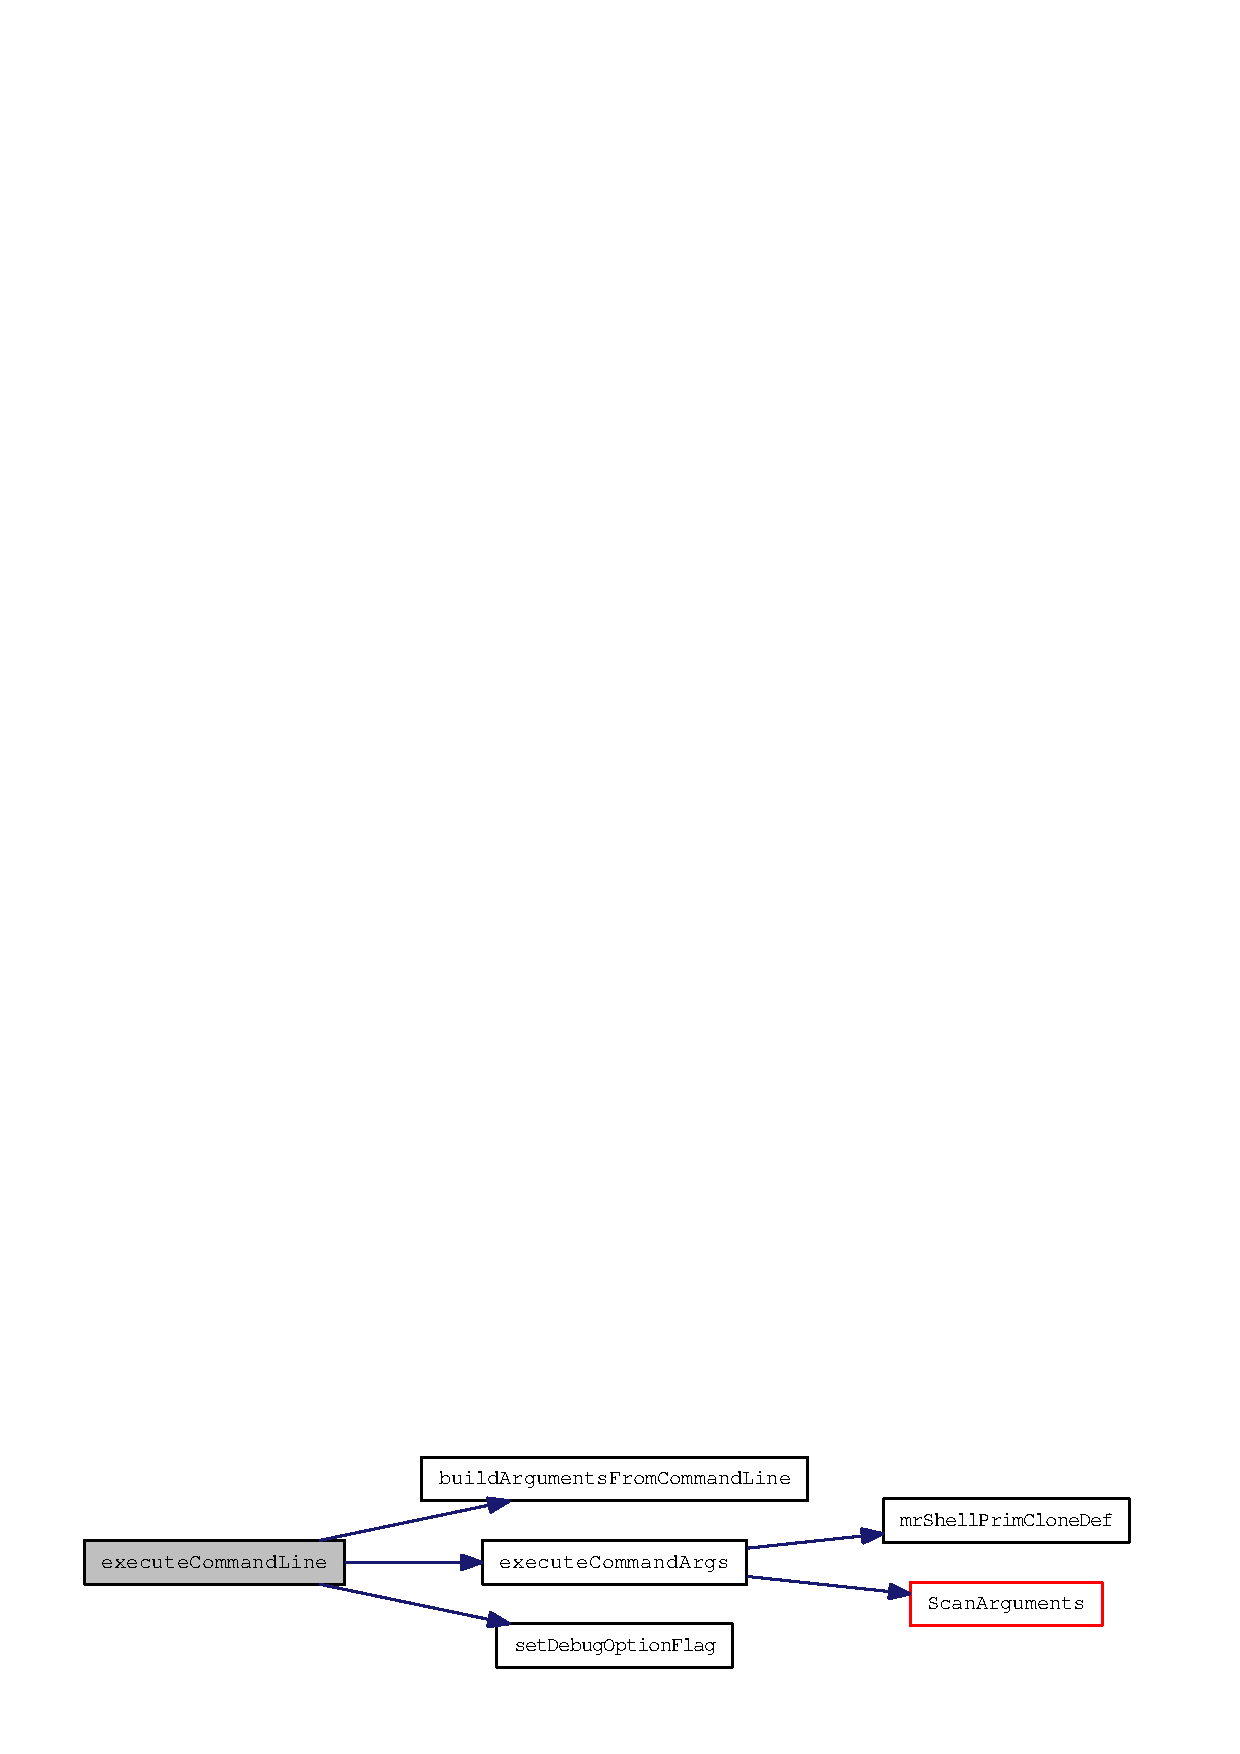
\includegraphics[width=273pt]{cmdInterpreter_8h_48086998882e7d163126de4100aa12ac_cgraph}
\end{center}
\end{figure}
\hypertarget{cmdInterpreter_8h_f03f7609a66def2e7fae02a477c38d97}{
\index{cmdInterpreter.h@{cmd\-Interpreter.h}!printHelp@{printHelp}}
\index{printHelp@{printHelp}!cmdInterpreter.h@{cmd\-Interpreter.h}}
\subsubsection[printHelp]{\setlength{\rightskip}{0pt plus 5cm}int print\-Help ()}}
\label{cmdInterpreter_8h_f03f7609a66def2e7fae02a477c38d97}




Definition at line 198 of file cmd\-Interpreter.c.

Referenced by execute\-Main\-Commands().\hypertarget{cmdInterpreter_8h_ac3ae2fb745e63e33060d5c0b658f745}{
\index{cmdInterpreter.h@{cmd\-Interpreter.h}!printInfo@{printInfo}}
\index{printInfo@{printInfo}!cmdInterpreter.h@{cmd\-Interpreter.h}}
\subsubsection[printInfo]{\setlength{\rightskip}{0pt plus 5cm}int print\-Info ()}}
\label{cmdInterpreter_8h_ac3ae2fb745e63e33060d5c0b658f745}




Definition at line 164 of file cmd\-Interpreter.c.\hypertarget{cmdInterpreter_8h_ae37490e691f5b4d2c2e8f22713555da}{
\index{cmdInterpreter.h@{cmd\-Interpreter.h}!terminateBatchProcessing@{terminateBatchProcessing}}
\index{terminateBatchProcessing@{terminateBatchProcessing}!cmdInterpreter.h@{cmd\-Interpreter.h}}
\subsubsection[terminateBatchProcessing]{\setlength{\rightskip}{0pt plus 5cm}int terminate\-Batch\-Processing ()}}
\label{cmdInterpreter_8h_ae37490e691f5b4d2c2e8f22713555da}




Definition at line 1280 of file cmd\-Interpreter.c.

References g\_\-b\-Batch\-Processing.

Referenced by sigquit\-Handler().